\documentclass[10pt,a4paper]{paper}
\usepackage[latin1]{inputenc}
\usepackage{amsmath}
\usepackage{amsfonts}
\usepackage{amssymb}
\usepackage{graphicx}
\usepackage{fancyvrb}
\usepackage[a4paper, total={7in, 8in}]{geometry}
\title{Introduction WIOD R package}
\author{Sybren Deuzeman}

\begin{document}
	\maketitle
	
	\section{Introduction}
	
	\section{Load International Input Output Tables}
	
	To be able to work with international input-output tables, we first need to load them into our program. There are two ways to do so: the first is to load the international input-output tables automatically into R. The other is to first make a local copy and then load it into R. The first method is useful if you either have a very strong internet connection or want to try the package. The second method is useful if you want to use the package intensively and do not want to download a lot of data every time you use the package. We first explain how to load international input-output tables from the internet. After that, we explain how to make a local copy and use that local copy.
	
	\subsection{Load from the Internet}
	
	To load data, one can use again two methods. The first one is loading a single international input output table. The second one is to load a set of input output tables into a list. The second method is most appropriate for executing the calculations on a set of input output tables, while the first one is most useful in creating your own personal methods with international input-output tables. We first explain how to load a single IOT and what the contents are, then we continue with loading the set of input-output tables. 
	
	\subsubsection{Single IOT}
	
	To load the World Input Output Database 2016 edition international input-output table for 2000, simply use
	\begin{verbatim}
		iot <- load_iot("WIOD2016", 2000)
	\end{verbatim}
	This will create the object iot, which is a large list. The list provided here is the basic building block of the package. These lists provide us with a way to make methods created with one version of the international input-output table compatible for use with other versions. The content of this list are shown in figure \ref{fig:contentiot} and is as follows:
	\begin{itemize}
		\item \texttt{I}: this is the block that describes the use of intermediate inputs from one industry being used by the other industry.
		\item \texttt{FD}: this contains data on the final demand used by other sectors. The $S$ block is the gross output of the industries.
		\item \texttt{VA}: is the value added by those industries. After that follow some parameter that can be used by the program.
		\item \texttt{c} is the number of countries in the input-output table
		\item \texttt{cf}: is number of countries for which we have data to which final demand goes.
		\item \texttt{n}: is the number of industries. 
		\item \texttt{f}: is the number of final demand categories. 
		\item \texttt{year}: is the year for which the international input-output table is.
		\item \texttt{version}: is the version of the international input-output table.
		\item \texttt{countries}: gives the countries in the order in which they appear in the input-output table.
		\item \texttt{industries}: gives the industries in the order in which they appear in the input-output table.
	\end{itemize}
	
	\begin{figure}[t]
	\centering
	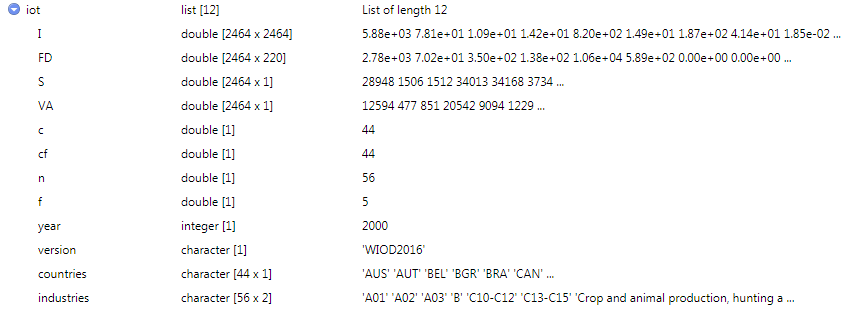
\includegraphics[width=\linewidth]{content_iot}
	\caption{The content of a Input-Output Table after loading it}
	\label{fig:contentiot}
	\end{figure}

	The main idea of the package are that multiple versions are available. At the moment, three versions of international input output tables are available: the World Input Output Database (WIOD) from 2013 and 2016 and the Inter-Country Input-Output Tables (ICIOT) from 2018 of the OECD. To access other versions or other years, for example the Inter-Country Input-Output Tables of the OECD for 2005, simply use	
	\begin{verbatim}
		iot_iciot <- load_iot("ICIOT", 2005)
	\end{verbatim}
	
	\subsubsection{List of IOTs}
	Especially for calculation purposes, loading in a list of international input-output tables is advisable. The package comes with some functions that automatically executes a function for a single IOT over all the IOTs in such a list. Also, the functions to extract the calculated data from the input-output tables uses these lists. To load in the complete set of international input-output tables from the 2016 edition into such a list, simply use:
	\begin{verbatim}
		WIOD2016 <- load_iots("WIOD2016").
	\end{verbatim}
	If you want to only load the international input-output tables for some specific years, say from 2005 to 2010, use
	\begin{verbatim}
		WIOD2016_0510 <- load_iots("WIOD2016", 2005:2010)
	\end{verbatim}
	
	\subsection{Make a Local Copy}
	
	\subsection{Load Extra Data}
	In some cases, extra data needs to be downloaded. For example, the WIOD project has also Socio-Economic Accounts. This data can be quite easily added to our list via either the \texttt{load\_extra\_iot} or \texttt{load\_extra\_iots} command. To load the Socio-Economic Accounts (SEA), one simply uses the following code for an already loaded iot:
	\begin{verbatim}
		iot <- load_extra_iot(iot, "SEA")
	\end{verbatim}
	This will add another list to the list with all data from the Socio-Economic Account. 
	To load the Socio-Economic Accounts to a list of IOTs, simply use
	\begin{verbatim}
		WIOD2016 <- load_extra_iots(WIOD2016, "SEA")
	\end{verbatim}
	
	
	\section{Use International Input Output Tables}
	To use the loaded Input-Output Tables to generate new measures, one can use some build-in functions on both a single IOT and on a list of multiple IOTs. We start again with the case of a single IOT to show what the package does in these cases. We first explain how to use the package with a single IOT and then with a list of multiple IOTs.
	
	\subsection{Use of package with single IOT}
	We use the build-in function GII, which calculates the global import intensity as in [[CITATION]] on the already loaded international input-output table $iot$. The code for this is:
	\begin{verbatim}
		iot <- gii(iot)
	\end{verbatim}
	Note that the output of this function need to be stored again. As done here, it can be stored again in the same object that is used to calculate. It can be stored in a new list, which will be a copy of the old list with the new calculations added.
	\begin{figure}
	\centering
	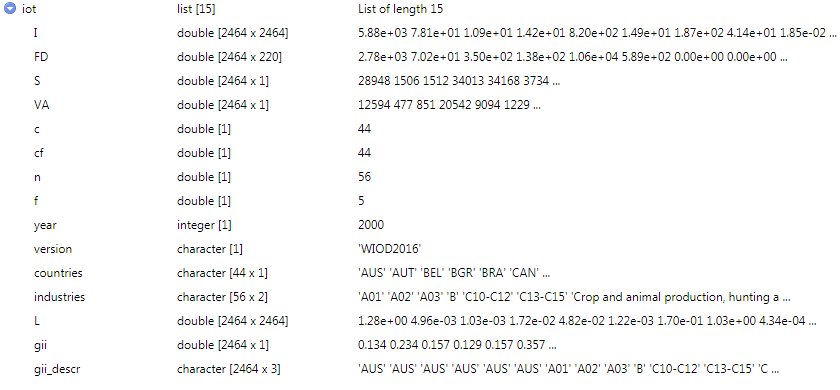
\includegraphics[width=1\linewidth]{content_iot_function}
	\caption{Content of \texttt{iot} after the command}
	\label{fig:contentiotfunction}
	\end{figure}

	Figure \ref{fig:contentiotfunction} shows the contents of \texttt{iot} after we have used this function. Compared to before, three things. The first is \texttt{L}, which is the Leontief inverse. Finding the Leontief inverse involves inversing a, in this case, 2464 by 2464, matrix. That operation takes a considerable amount of time and we avoid that by storing the Leontief Inverse for later use. The second element that is added is \texttt{gii}, which stores the calculations. The third added element is \texttt{gii\_descr}, which describes for which country and sector that data is applicable. The third element will be used when we export the results.
	
	The function \texttt{gii} also allows for two other arguments, namely \texttt{regions} and \texttt{industries}. These arguments add region and industry categories to \texttt{gii\_descr}. To get an appropriate categorization, one can use the function \texttt{countrycat}. To add a NAFTA and BeNeLux categorization, one can use
	\begin{verbatim}
		NAFTA <- c("USA", "MEX", "CAN")
		BENELUX <- c("BEL", "NLD", "LUX") 
		regions <- countrycat(list(NAFTA, BENELUX), iots)
	\end{verbatim} 
	to create a region categorization. Finally, one can use
	\begin{verbatim}
		iot <- gii(iot, regions = regions)
	\end{verbatim}
	to include the region categories to the data description.
	
	\subsection{Use of package with set of IOTs}
	To execute $gii$ on the set of IOTs we have loaded before, we can use another function, namely \texttt{on\_iots}\footnote{\texttt{on\_iots} is basically the one-liner \texttt{iots <- lapply(iots, fun, ...)}.}. The function \texttt{on\_iots} executes a function on all the input-output tables in the list and the command to do so for the function \texttt{gii} on our list of IOTs \texttt{WIOD2016} is:
	\begin{verbatim}
		WIOD2016 <- on_iots(gii, WIOD2016)
	\end{verbatim}
	To add extra arguments, like te region categories, you can add these as extra arguments to \texttt{on\_iots}:
	\begin{verbatim}
	WIOD2016 <- on_iots(gii, WIOD2016, regions = regions)
	\end{verbatim}
	
	\section{Export Results}
	As explained before the results are stored in a list of lists. In this way, it is not easy to use our results elsewhere for further analysis. To extract the results from this list of lists, we can use two functions: \texttt{export\_dataframe} and \texttt{export\_csv}. The first function exports the data to an R dataframe. The second function exports the data into a CSV file.
	\subsection{Export into a Dataframe}
	
	To extract the global import intensities from \texttt{WIOD2016} into a dataframe, we can use:
	\begin{verbatim}
		gii_df <- export_dataframe("gii", WIOD2016)
	\end{verbatim}
	This generates a dataframe in ``wide'' format. For every year, there is a separate column. We can also export the data into ``long'' format, in which year is just another variable. To do so, we can use:
	\begin{verbatim}
		gii_df_long <- export_dataframe("gii", WIOD2016, long = TRUE)
	\end{verbatim}
	To add, for example, the total final demand for certain sectors, one can do so as well
	\begin{verbatim}
		WIOD2016 <- on_iots(fd_total, WIOD2016)
		gii_fvas_df <- export_dataframe(c("gii", "fd_total"), WIOD2016)
	\end{verbatim}	
	An error will occur when the outputs for \texttt{gii} and \texttt{fd\_total} are not of the same length. In this case, these however are of the same length, so that is not a problem. Note further that the data description for \texttt{gii} will be used as it is the first in the list.
	
	\subsection{Export into a CSV file}
	The function \texttt{export\_csv} has the same basic setup, although it does not store a dataframe within R. The most simple way is
	\begin{verbatim}
		export_csv("gii", WIOD2016)
	\end{verbatim}
	If one runs this code, a prompt window will open to ask where to store the results. That information can also be added in the code using the directory argument like this:
	\begin{verbatim}
		export_csv("gii", WIOD2016, directory = "C://Some/Dir/and/File.csv")
	\end{verbatim}
	\section{Make Your Own Functions}
	The strength of this package is that you only need to write the function, while the rest of the package takes care of managing the data. The functions can be written such that they function with a single input-output table. Using this for all years and for other versions of international input-output tables is taken care of by the WIOD package.
	
	To aid in writing your own functions, we add among the simplest, but still complete functions in our package: the \texttt{gii} function
	\begin{Verbatim}
	gii <- function(iot, regions = "None", industries = "None"){
		# Obtain some necessary preliminary calculations
		A <- coefficient(iot)
		iot <- leontief(iot)
	
		# Get results
		temp = matrix(1, iot$c, iot$c) # Create a c x c matrix with ones
		for (i in 1:iot$c){
			temp[i,i]=0 # make the diagonal into 0's
		}
		S = kronecker(temp, matrix(1, iot$n, iot$n)) 
		result <- t(colSums(S * A) %*% iot$L) 
		
		# Store results to the list
		iot$gii <- result	
		iot$gii_descr <- countryindustry_descr(iot, regions, industries)
		
		# Return the list
		return(iot)
	}	
	\end{Verbatim}
	First, we do some necessary calculations: namely the coefficient matrix \texttt{A} and the Leontief matrix \texttt{L}. Observe that we do not store the coefficient matrix into the input-output table, but we do store the Leontief matrix. Calculating the coefficient matrix is fast, while it is a large matrix to store. The Leontief matrix is as large to store, but calculating it takes a considerable amount of time.
	
	Next, we do some calculations to get the necessary results. Observe that we use \texttt{colSums()}, which gives the sum of all columns. In R, most matrix manipulations are not very efficient, while element-wise manipulation is much faster. In contrast with MatLab, it is therefore advisable to avoid the use of matrix manipulation as much as possible. Finally, the results are stored using \texttt{iot\$gii <- result}. We add a description via \texttt{iot\$gii\_descr <- countryindustry\_descr(iot, regions, industries)}. This list is then being returned from the function.
	\end{document}